\section{Resultados}
\label{sec:resultados}

\subsection{Viés Estrutural nas Bases de Dados}

Antes de qualquer modelagem, o viés presente em cada base já revela diferenças substanciais entre as séries PD e GS (Figura~\ref{fig:vies_original}). Na série PD, o abs\_SPD cresce de forma contínua de 0.20 ($v=0$) a 0.87 ($v=1$), e o DI cai de 1.28 a 0.13: na base mais enviesada, o grupo desprivilegiado recebe predição favorável com frequência oito vezes menor que o grupo privilegiado. Na série GS, o viés introduzido é estruturalmente diferente: abs\_SPD oscila entre 0.06 e 0.23, com DI sempre próximo de 1.0 nas versões com menor viés. A base \texttt{gs\_v1} contém apenas um grupo sensível, inviabilizando o cálculo das métricas de equidade e por isso está ausente dos gráficos desta seção. Esse contraste entre séries impõe um desafio para a generalização dos modelos: um classificador treinado em PD enfrenta distribuições de grupo muito mais assimétricas do que quando treinado em GS.

\begin{figure}[H]
    \centering
    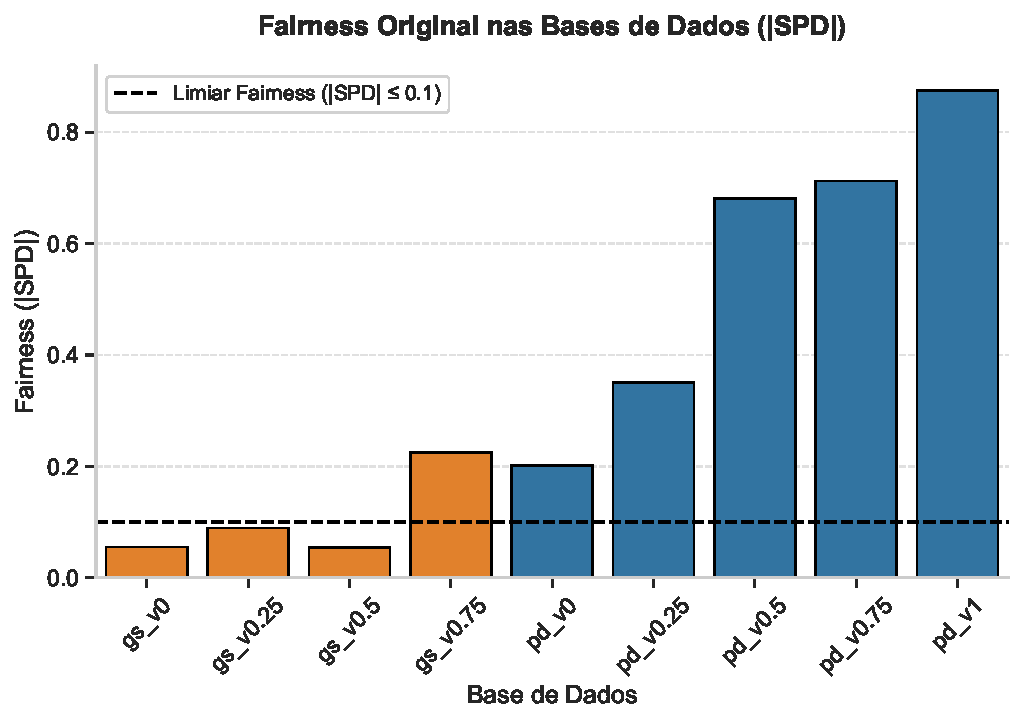
\includegraphics[width=0.48\textwidth]{figures/fig01a_vies_original_spd.pdf}
    \hfill
    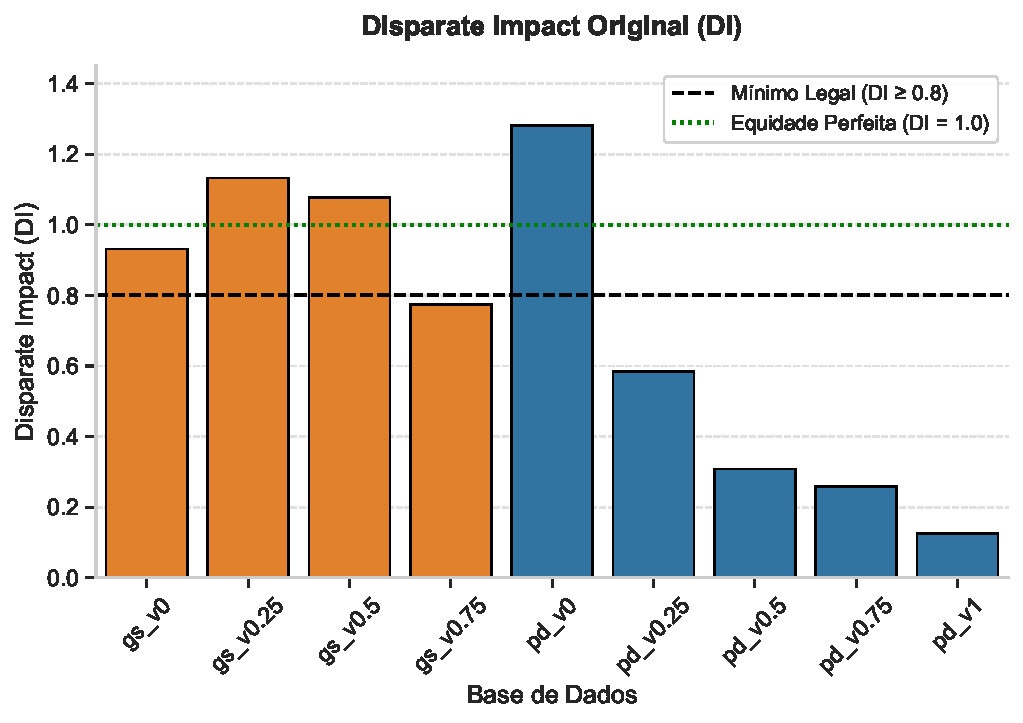
\includegraphics[width=0.48\textwidth]{figures/fig01b_vies_original_di.pdf}
    \caption{Viés nos dados brutos de cada base (abs\_SPD e DI) antes do
    treinamento, por série e nível de viés controlado. A base
    \texttt{gs\_v1} é omitida por conter apenas um grupo sensível,
    o que inviabiliza o cálculo das métricas de equidade.}
    \label{fig:vies_original}
\end{figure}

\subsection{Efeito do Parâmetro \texorpdfstring{$\eta$}{eta} do Prejudice Remover}
\label{sec:eta}

A Figura~\ref{fig:eta} apresenta o comportamento de F1 e abs\_SPD ao longo da varredura de $\eta \in \{0.0;\; 1.0;\; 5.0;\; 10.0;\; 15.0;\; 25.0;\; 35.0;\; 50.0\}$. Com $\eta = 0$, equivalente a uma Regressão Logística sem penalidade de equidade, o modelo atingiu F1~$= 0.9911$ e abs\_SPD~$= 0.358$, com DI~$= 0.719$. À medida que $\eta$ cresce, o F1 diminui constantemente: em $\eta = 10$ cai para 0.910; em $\eta = 25$, para 0.894; e em $\eta = 50$, para 0.834. O abs\_SPD acompanha essa trajetória com algumas oscilações, atingindo o valor mínimo de 0.278 em $\eta = 50$ (DI~$= 0.776$), redução de 22.3\% em relação ao modelo base. A regra dos quatro quintos (DI~$\geq 0.8$) não foi atingida em média para nenhum valor de $\eta$.

\begin{figure}[H]
    \centering
    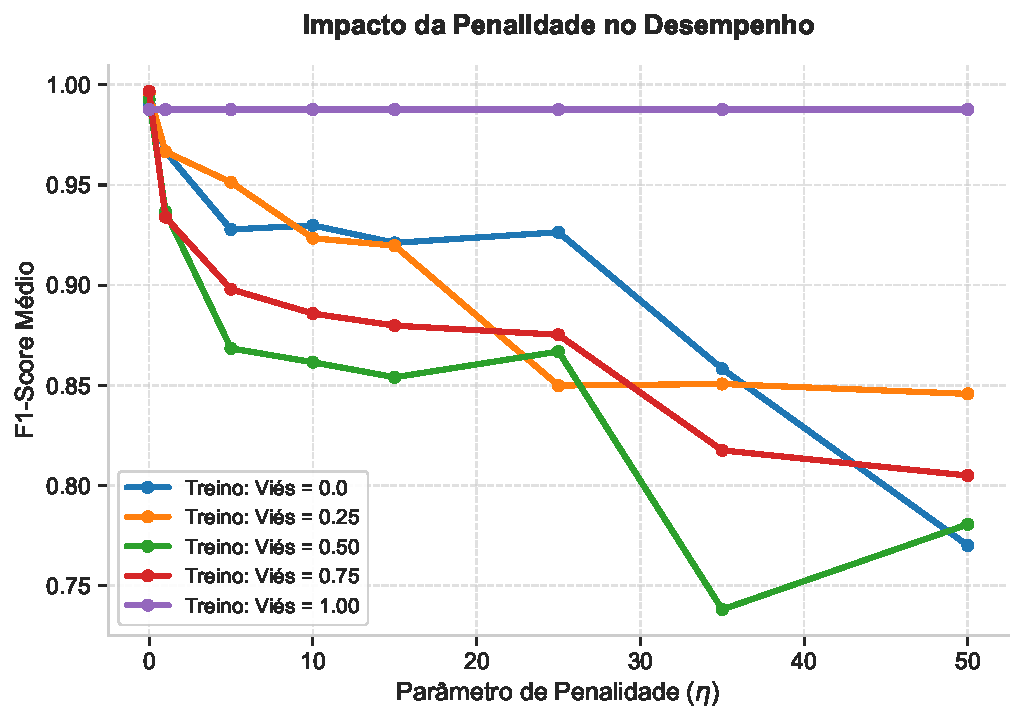
\includegraphics[width=0.48\textwidth]{figures/fig02a_f1_eta.pdf}
    \hfill
    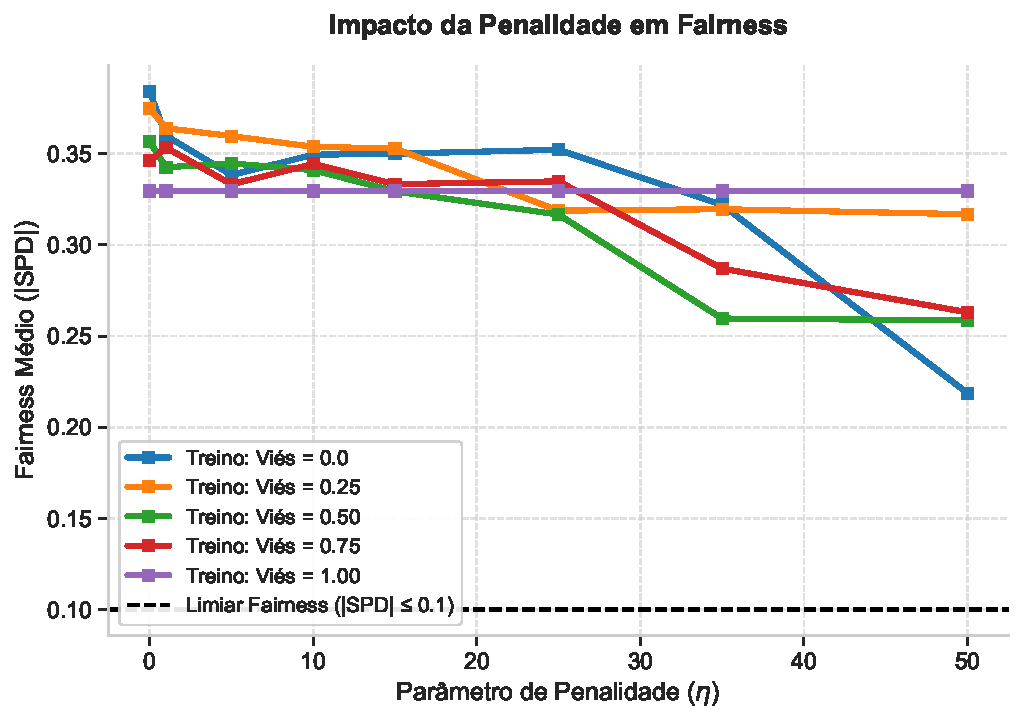
\includegraphics[width=0.48\textwidth]{figures/fig02b_spd_eta.pdf}
    \caption{F1-Score e abs\_SPD em função do parâmetro $\eta$ do
    Prejudice Remover, médias sobre todos os pares treino--teste. Cada curva corresponde a um nível de viés da base de treinamento.}
    \label{fig:eta}
\end{figure}

O comportamento diverge acentuadamente entre séries. Na série GS, $\eta$ elevado produziu ganhos mínimos de equidade: entre $\eta = 0$ e $\eta = 50$, abs\_SPD caiu apenas de 0.382 para 0.364 (-4.7\%), enquanto F1 caiu de 0.994 para 0.966 (-2.8\%). Já na série PD, a resposta ao regularizador foi muito mais intensa: abs\_SPD reduziu de 0.334 para 0.190 (-43\%), mas F1 sofreu queda de 0.989 para 0.702 (-29\%). Exclusivamente na série PD com $\eta = 50$, o DI médio atingiu 0.855, ultrapassando o limiar de 0.8. Os heatmaps da Figura~\ref{fig:heatmaps} mostram como essa diferença se manifesta nas combinações individuais de bases de treinamento e teste. As células com maior abs\_SPD correspondem a pares nos quais a base de treinamento tem viés elevado e a base de teste tem distribuição de grupos distinta, evidenciando que o modelo aprende e transfere o padrão desigual do dado de origem.

\begin{figure}[H]
    \centering
    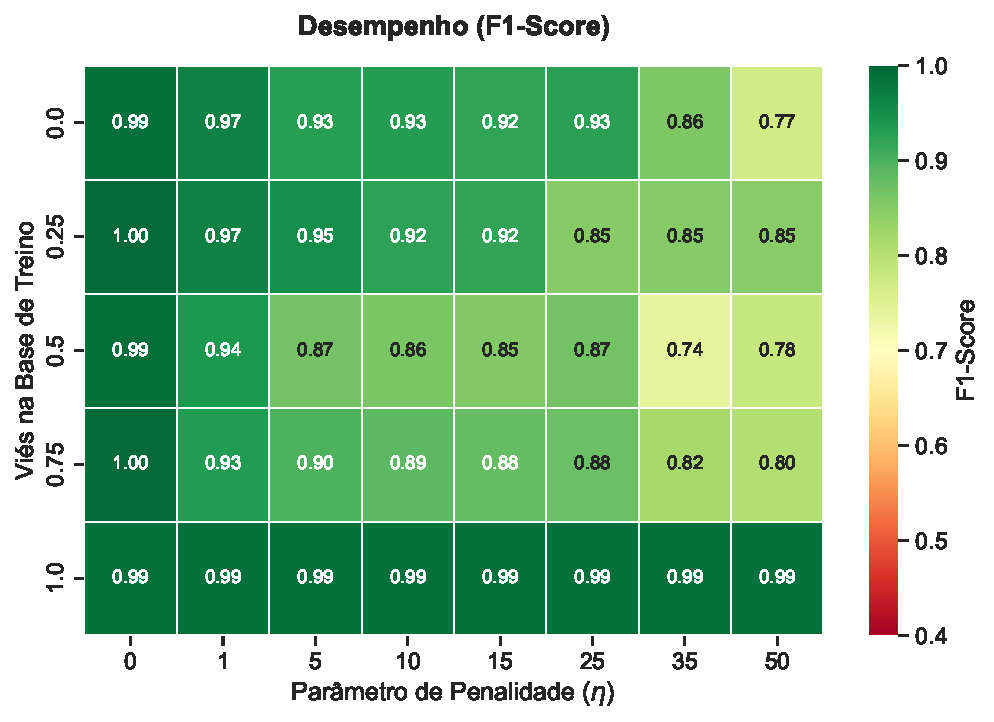
\includegraphics[width=0.48\textwidth]{figures/fig03a_heatmap_f1.pdf}
    \hfill
    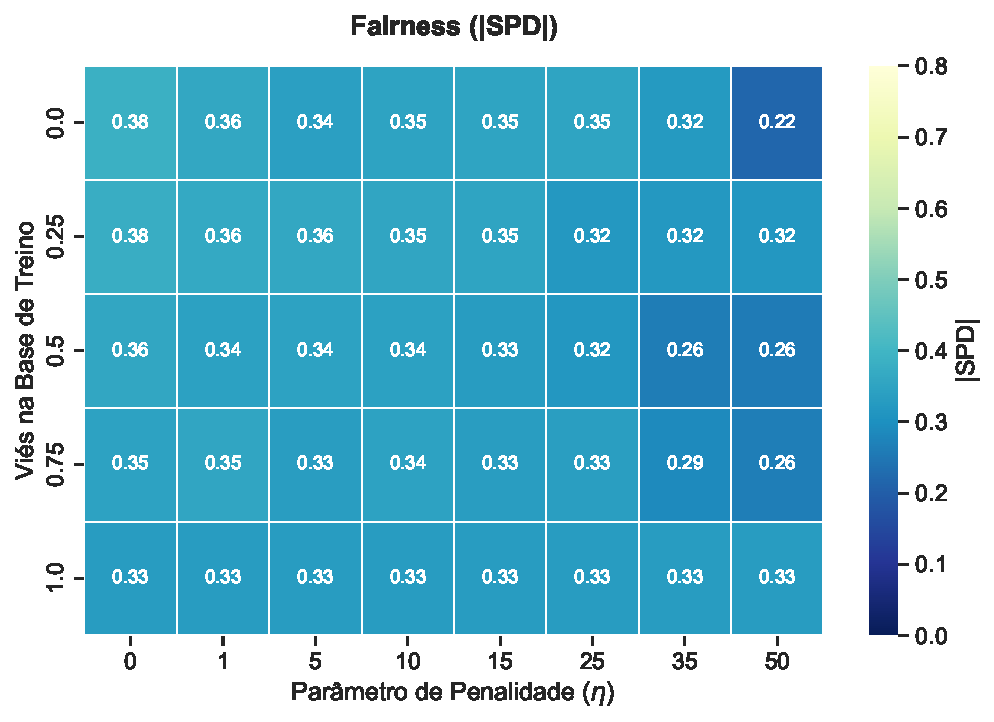
\includegraphics[width=0.48\textwidth]{figures/fig03b_heatmap_spd.pdf}
    \caption{Heatmaps de F1-Score e abs\_SPD por nível de viés da base
    de treinamento versus parâmetro $\eta$, médias sobre todas as bases
    de teste. Valores mais claros no heatmap de abs\_SPD indicam maior
    disparidade.}
    \label{fig:heatmaps}
\end{figure}

A comparação direta entre $\eta = 0$ e $\eta = 35$ na Figura~\ref{fig:matrizes} ilustra a troca entre desempenho e equidade: à medida que o regularizador avança, as células de maior abs\_SPD escurecem de forma não uniforme. Certas combinações de bases respondem bem à penalidade, enquanto outras permanecem praticamente inalteradas, evidenciando que a capacidade do Prejudice Remover depende fortemente do viés estrutural da base de treinamento.

\begin{figure}[H]
    \centering
    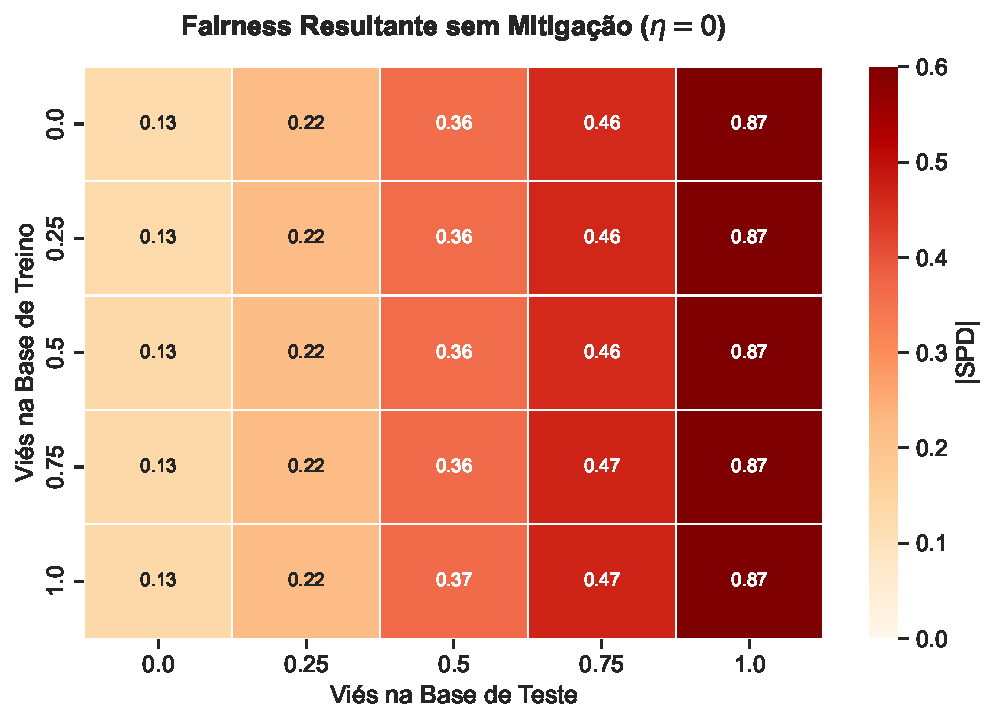
\includegraphics[width=0.48\textwidth]{figures/fig04a_matriz_vies_eta0.pdf}
    \hfill
    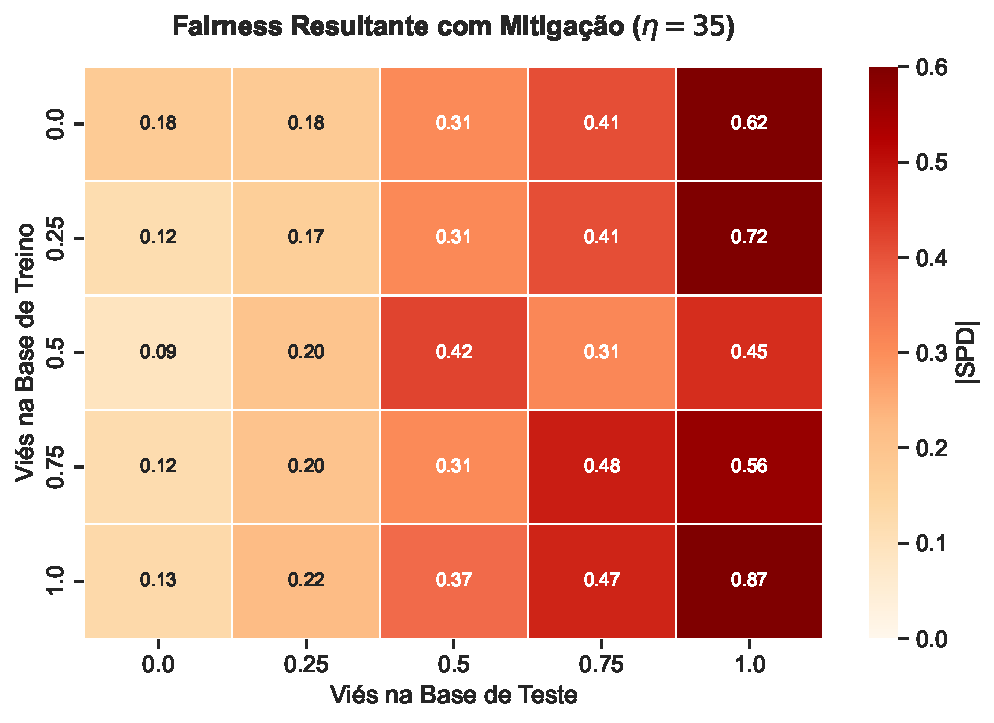
\includegraphics[width=0.48\textwidth]{figures/fig04b_matriz_vies_eta35.pdf}
    \caption{Matrizes de abs\_SPD por par de bases (viés treino $\times$
    viés teste) para $\eta = 0$ (esquerda) e $\eta = 35$ (direita). A
    redução de disparidade é mais expressiva nas bases PD com alto viés
    de treinamento; as combinações envolvendo GS respondem pouco ao
    regularizador.}
    \label{fig:matrizes}
\end{figure}

A Figura~\ref{fig:metricas_eta} detalha a degradação simultânea de recall, precisão e F1 conforme $\eta$ aumenta. O recall se mantém mais estável que a precisão: em $\eta = 50$, recall~$= 0.893$ frente a precisão~$= 0.782$, sugerindo que o regularizador torna o modelo mais cauteloso na sinalização de fraude sem perder tanto na detecção de casos reais.

\begin{figure}[H]
    \centering
    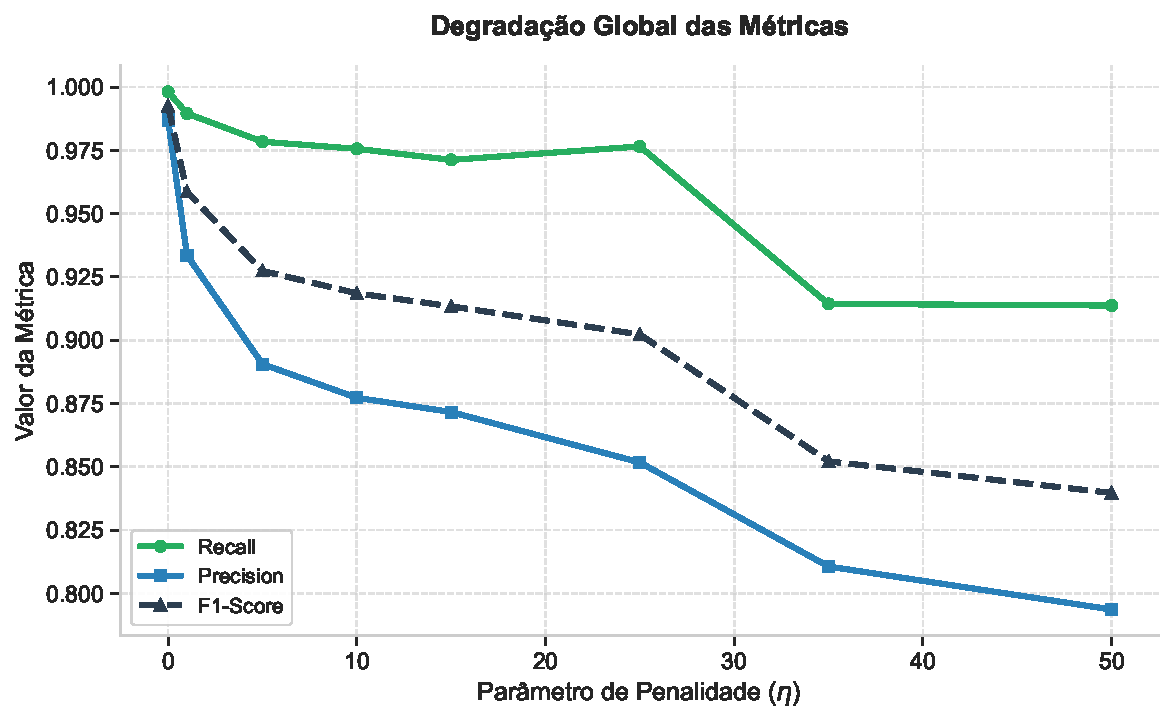
\includegraphics[width=0.72\textwidth]{figures/fig05_metricas_classificacao.pdf}
    \caption{Degradação global de recall, precisão e F1-Score em função
    de $\eta$. O recall decresce mais lentamente que a precisão,
    indicando que a penalidade de equidade afeta principalmente a
    tendência do modelo de sinalizar transações como fraudulentas.}
    \label{fig:metricas_eta}
\end{figure}

Por fim, a capacidade de generalização do modelo frente a diferentes distribuições de viés também é afetada pelo regularizador. A Figura~\ref{fig:generalizacao} ilustra o comportamento para F1-Score e abs\_SPD ao longo do parâmetro $\eta$, separando os resultados entre predições feitas na mesma série da base original e predições feitas em uma série distinta. Fica evidente que o viés aprendido generaliza de forma assimétrica: modelos avaliados em séries diferentes daquelas em que foram treinados apresentam disparidade consistentemente maior.

\begin{figure}[H]
    \centering
    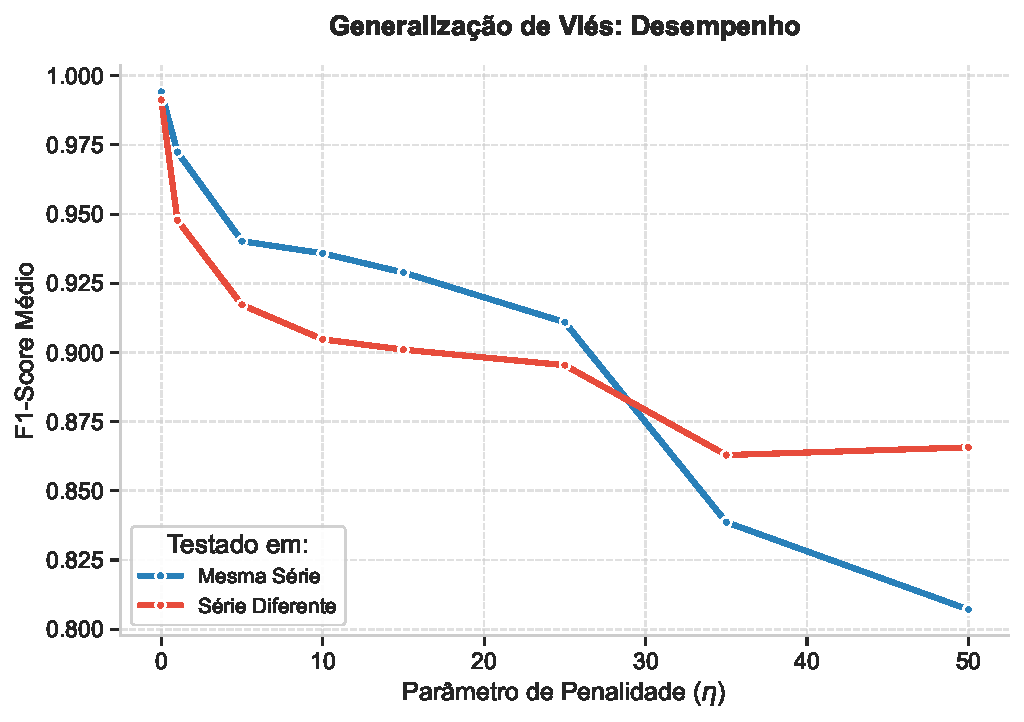
\includegraphics[width=0.48\textwidth]{figures/fig08a_generalizacao_f1.pdf}
    \hfill
    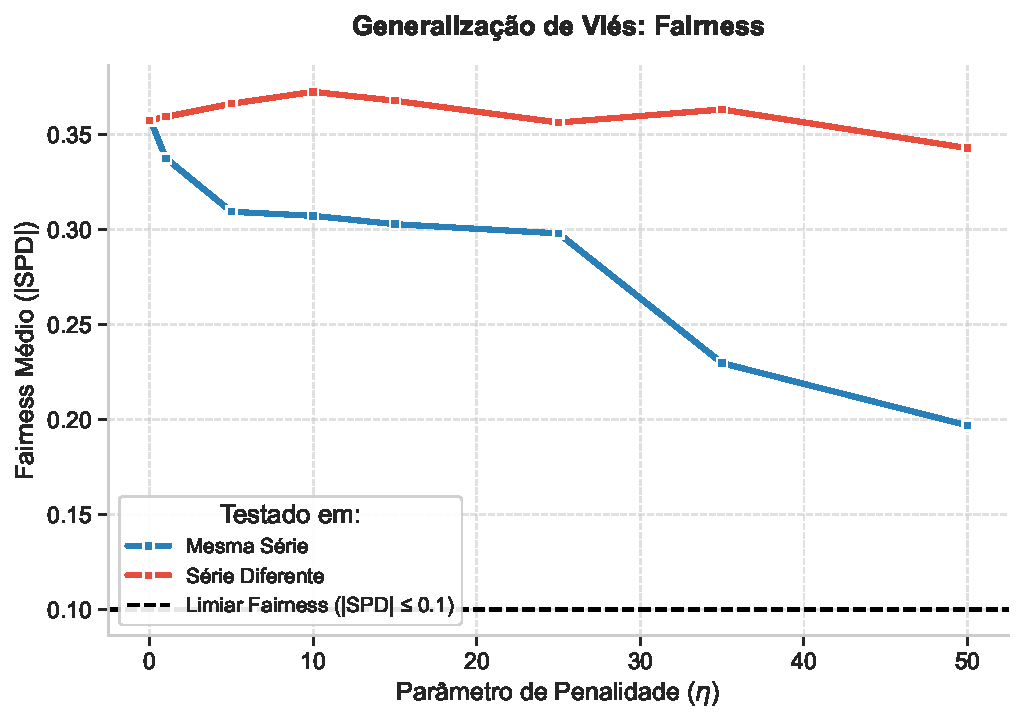
\includegraphics[width=0.48\textwidth]{figures/fig08b_generalizacao_spd.pdf}
    \caption{F1-Score e abs\_SPD em função do parâmetro $\eta$,
    desagregados pelo cruzamento de séries: modelos avaliados na mesma
    série de origem versus avaliados em uma série distinta. Pares de
    séries distintas tendem a apresentar maior disparidade, evidenciando
    que o viés aprendido generaliza de forma assimétrica entre PD e GS.}
    \label{fig:generalizacao}
\end{figure}

\subsection{Efeito do Volume de Dados de Treinamento}
\label{sec:volume}

A Tabela~\ref{tab:volume} reúne as médias globais para os cinco volumes testados. O F1 cresceu de 0.9777 (1.000 amostras) a 0.9911 (10.000 amostras), ganho de apenas 0.0134, menos de 1.4\% relativo. A precisão acompanhou esse crescimento de forma mais consistente (+0.025), enquanto o recall permaneceu estável (variação $< 0.001$). Esse padrão sugere que, a partir de aproximadamente 1.000 amostras balanceadas, o modelo já captura os principais padrões preditivos; volume adicional refina a precisão em casos marginais sem ampliar substancialmente a detecção.

\begin{table}[H]
\centering
\caption{Médias globais por volume de treinamento (Regressão Logística
balanceada, 10 features).}
\label{tab:volume}
\begin{tabular}{rrrrrrr}
\toprule
\textbf{Volume} & \textbf{F1} & \textbf{Precision} & \textbf{Recall}
  & \textbf{abs\_SPD} & \textbf{DI} \\
\midrule
1.000  & 0.9777 & 0.9593 & 0.9972 & 0.3515 & 0.7225 \\
2.500  & 0.9837 & 0.9702 & 0.9977 & 0.3548 & 0.7206 \\
5.000  & 0.9882 & 0.9784 & 0.9982 & 0.3569 & 0.7196 \\
7.500  & 0.9899 & 0.9820 & 0.9981 & 0.3575 & 0.7193 \\
10.000 & 0.9911 & 0.9844 & 0.9980 & 0.3580 & 0.7190 \\
\bottomrule
\end{tabular}
\end{table}

No eixo da equidade, o resultado é contra-intuitivo: abs\_SPD aumentou de 0.3515 para 0.3580 (+0.0065) à medida que o volume cresceu, e o DI afastou-se de 1.0 no mesmo sentido. Mais dados não corrigiram o viés aprendido; ao contrário, o modelo reproduziu com maior fidelidade os padrões desiguais presentes nos dados. 

Um achado adicional merece atenção: com 10.000 amostras, bases de treinamento com maior viés sintético produziram F1 mais alto (v~$= 0.75$: F1~$= 0.9958$) do que bases sem viés (v~$= 0.00$: F1~$= 0.9886$). O viés introduzido aumenta a separabilidade entre classes no conjunto de treinamento, facilitando a tarefa preditiva, mas ao custo de abs\_SPD mais elevado nas predições (v~$= 0.00$: 0.384; v~$= 0.75$: 0.346), pois os modelos treinados em dados mais enviesados tendem a generalizar esse viés para os conjuntos de teste.

\subsection{Efeito do Conjunto de Atributos}
\label{sec:features}

A Tabela~\ref{tab:features} apresenta os resultados para os quatro conjuntos de features. O salto mais expressivo ocorreu na transição de \texttt{transacional\_2} para \texttt{tipo\_temporal\_4}: F1 subiu de 0.5322 para 0.9701 (+0.438), inteiramente conduzido pela adição de \texttt{is\_cnab220}. Transações de crédito (CNAB~$= 220$) concentram quase toda a fraude na base, tornando essa feature um preditor próximo de determinístico. Sem ela, o modelo operou com recall alto (0.9698) mas precisão drasticamente reduzida (0.3689), classificando a maioria das transações como fraude indiscriminadamente.

\begin{table}[H]
\centering
\caption{Médias globais por conjunto de atributos (Regressão Logística
balanceada, N~$= 10.000$).}
\label{tab:features}
\begin{tabular}{lrrrrr}
\toprule
\textbf{Conjunto} & \textbf{F1} & \textbf{Precision} & \textbf{Recall}
  & \textbf{abs\_SPD} & \textbf{DI} \\
\midrule
\texttt{transacional\_2}   & 0.5322 & 0.3689 & 0.9698 & 0.1866 & 0.7877 \\
\texttt{tipo\_temporal\_4} & 0.9701 & 0.9428 & 0.9993 & 0.3548 & 0.7175 \\
\texttt{comportamental\_6} & 0.9844 & 0.9697 & 0.9997 & 0.3610 & 0.7145 \\
\texttt{completo\_10}      & 0.9911 & 0.9844 & 0.9980 & 0.3580 & 0.7190 \\
\bottomrule
\end{tabular}
\end{table}

As transições seguintes produziram retornos decrescentes. A adição das features comportamentais do titular (\texttt{tipo\_temporal\_4} $\to$ \texttt{comportamental\_6}) acrescentou 0.014 de F1 e 0.027 de precisão, com recall quase inalterado. A inclusão dos z-scores por ramo (\texttt{completo\_10}) contribuiu mais 0.007 de F1 e 0.015 de precisão, com leve queda de recall (-0.002). A normalização por ramo remove parte do efeito de grupo nas features, melhorando a generalização entre bases com distribuições distintas.

No eixo da equidade, o padrão foi não monótono. O conjunto \texttt{transacional\_2} apresentou o menor abs\_SPD (0.187), mas esse valor reflete a precisão colapsada, não equidade genuína: quando o modelo classifica quase tudo como fraude, a diferença entre grupos encolhe por indiferença. A adição de \texttt{is\_cnab220} elevou o abs\_SPD para 0.355, porque o modelo passou a diferenciar grupos de forma efetiva. Os dois conjuntos maiores oscilaram entre 0.355 e 0.361, sem tendência clara, confirmando que atributos adicionais não mitigam o viés estrutural dos dados.

\subsection{Comparação de Métodos de Mitigação}
\label{sec:mitigacao}

A Tabela~\ref{tab:mitigacao} compara os quatro métodos sobre o conjunto de 9 features (sem \texttt{is\_cnab220}, cuja presença tornaria o problema preditivo quase trivial).

\begin{table}[H]
\centering
\caption{Médias globais por método de mitigação (9 features,
N~$= 10.000$).}
\label{tab:mitigacao}
\begin{tabular}{lrrrrr}
\toprule
\textbf{Método} & \textbf{F1} & \textbf{Precision} & \textbf{Recall}
  & \textbf{abs\_SPD} & \textbf{DI} \\
\midrule
LR sem mitigação              & \textbf{0.9663} & \textbf{0.9615} & 0.9718 & 0.3425 & 0.7271 \\
LR balanceado                 & 0.9616 & 0.9398 & 0.9850          & 0.3450 & 0.7252 \\
LR reponderado                & 0.9608 & 0.9374 & \textbf{0.9861} & 0.3433 & 0.7254 \\
Prejudice Remover ($\eta=10$) & 0.8857 & 0.8341 & 0.9599          & \textbf{0.3323} & 0.6970 \\
\bottomrule
\end{tabular}
\end{table}

O modelo sem balanceamento obteve o melhor F1 (0.9663) e a maior precisão (0.9615), porém o menor recall (0.9718) entre os métodos LR. Isso reflete o comportamento esperado: sem forçar equilíbrio entre classes, o modelo é mais conservador na sinalização de fraude. O abs\_SPD (0.3425) ficou abaixo do LR balanceado, resultado que indica que o balanceamento redistribui erros de forma simétrica entre classes, mas não entre grupos sensíveis.

O LR balanceado maximizou o recall (0.9850) entre os modelos LR, ao custo de menor precisão e F1. O abs\_SPD (0.3450) foi o mais alto dos quatro métodos, confirmando que o balanceamento por classe não reduz a disparidade de predição entre grupos.

A reponderação de Kamiran e Calders produziu resultados praticamente idênticos ao LR balanceado: F1 -0.0007, recall +0.0011 e abs\_SPD -0.0017. A diferença de equidade situou-se na terceira casa decimal, indicando que as duas abordagens de pré-processamento são intercambiáveis neste contexto.

O Prejudice Remover com $\eta = 10$ foi o único método a reduzir abs\_SPD de forma perceptível: 0.3323 (-0.013 em relação ao LR balanceado). Em contrapartida, F1 caiu para 0.8857 (-0.076) e precisão para 0.8341 (-0.106). O comportamento por nível de viés é não monótono: a maior redução de abs\_SPD ocorreu em $v = 0$ (-0.042 em relação ao LR balanceado), enquanto em $v = 0.75$ o ganho de equidade foi mínimo (-0.003) com queda de F1 de -0.114, o pior custo-benefício de todos os cenários. Em $v = 1.0$, o Prejudice Remover passou a atuar como LR puro (\textit{fallback} por ausência de grupos em algumas bases), produzindo resultado idêntico ao LR balanceado. A resposta ao regularizador também diferiu entre séries: a série PD respondeu com redução de F1 de 0.9572 para 0.8199 (-0.138) e redução de abs\_SPD de 0.3234 para 0.3099 (-0.014), enquanto a série GS cedeu apenas 0.0145 de F1 com redução de abs\_SPD de apenas 0.012. Nenhum método atingiu DI~$\geq 0.8$ em média.

\section{Discussão}
\label{sec:analises}

Os resultados permitem organizar as respostas às perguntas de pesquisa em torno de três eixos.

\textbf{Volume de dados.} A partir de 1.000 amostras balanceadas, o modelo já produziu F1~$= 0.977$, desempenho altamente competitivo. Volume adicional trouxe ganhos marginais e decrescentes em F1, sem nenhum benefício para a equidade; ao contrário, abs\_SPD cresceu de forma contínua com o volume (+0.007 de 1.000 a 10.000 amostras). O modelo simplesmente aprendeu os padrões desiguais com maior fidelidade à medida que mais exemplos foram fornecidos. Esse resultado, alinhado com os achados de~\citeonline{zhang2021ignorance} sobre o efeito do tamanho do conjunto de treinamento, indica que mais dados podem acentuar levemente o viés aprendido, e que um volume maior não implica automaticamente maior injustiça, mas também não corrige o viés estrutural.

\textbf{Seleção de atributos.} Adicionar features melhorou sistematicamente o F1, mas não reduziu o viés estrutural. O valor mínimo de abs\_SPD no conjunto \texttt{transacional\_2} decorreu da indiferença do modelo, não de equidade real. A partir da adição de \texttt{is\_cnab220}, o abs\_SPD estabilizou em torno de 0.355--0.361, independentemente de quantos atributos foram incluídos. Mais atributos não garantem maior justiça, e os ganhos de precisão não foram acompanhados por ganhos proporcionais de equidade. Isso contrasta com a conclusão de~\citeonline{zhang2021ignorance} de que conjuntos de features mais ricos tendem a reduzir o viés, diferença que pode ser atribuída ao caráter sintético e ao alto nível de correlação entre o atributo sensível e a variável alvo nas bases utilizadas.

\textbf{Métodos de mitigação.} O balanceamento melhorou recall, mas elevou ligeiramente o abs\_SPD em relação ao modelo não balanceado (+0.003), confirmando que o impacto na equidade é limitado e pode ser contraproducente. A reponderação ofereceu a melhor equidade entre os modelos LR, mas com diferença insignificante (-0.002 de abs\_SPD), e as melhorias não foram significativas. O Prejudice Remover foi a única técnica com redução perceptível de abs\_SPD (-0.013), mas com custo expressivo de F1 (-0.076) e comportamento errático por série e nível de viés. O limiar DI~$\geq 0.8$ não foi atingido por nenhum método em média, sendo alcançado apenas no subconjunto da série PD com $\eta = 50$, que ao mesmo tempo apresentou queda de F1 para 0.702.

Em conjunto, os resultados indicam que o viés observado nas predições é predominantemente estrutural, originado na correlação entre o atributo sensível e a variável alvo nos próprios dados, e resistente às técnicas de mitigação convencionais. Intervenções que não alteram essa correlação de base, como balanceamento e reponderação, produzem efeitos marginais. O Prejudice Remover, ao penalizar diretamente a dependência entre predições e grupo sensível, consegue reduções perceptíveis, mas à custa da performance preditiva e de forma inconsistente entre contextos.

\section{Conclusão}
\label{sec:conclusao}

Este trabalho investigou como o viés nos dados de treinamento e as escolhas de modelagem afetam a equidade de modelos de detecção de fraudes em transações financeiras. Três conjuntos de experimentos foram conduzidos sobre dez bases com viés sintético controlado, cobrindo perguntas de pesquisa relacionadas a volume de dados, seleção de atributos e técnicas de mitigação.

Os achados convergem para uma conclusão central: o viés de predição é estrutural e resistente às técnicas convencionais de mitigação. Aumentar o volume de dados não corrigiu a disparidade entre grupos, apenas a agravou levemente. Adicionar atributos melhorou a performance preditiva, mas não reduziu o abs\_SPD a partir do momento em que o modelo passou a distinguir os grupos de forma efetiva. Entre os métodos de mitigação, apenas o Prejudice Remover produziu redução perceptível de abs\_SPD, ao custo de queda expressiva de F1 e com comportamento inconsistente entre as séries PD e GS. Nenhum método atingiu o limiar DI~$\geq 0.8$ em média.

Esses resultados têm implicações práticas diretas: em domínios onde o viés está fortemente correlacionado com a variável alvo, como ocorre nas séries PD das bases utilizadas, intervenções de mitigação aplicadas apenas na etapa de modelagem têm alcance limitado. A correção do viés exige atenção desde a coleta e curadoria dos dados, incluindo estratégias de amostragem que garantam representação adequada dos grupos sensíveis em ambas as classes.